% !TEX root = saveliev_physics_general_course_1.tex
%!TEX TS-program = pdflatex
%!TEX encoding = UTF-8 Unicode


\chapter{CƠ HỌC TƯƠNG ĐỐI TÍNH}\label{chap:8}

\section{Thuyết tương đối hẹp}\label{sec:8_1}

Trong~\ref{sec:2_1} người ta đã nhận xét rằng cơ học Newton chỉ đúng đối với các vật chuyển động với các vận tốc nhỏ hơn vận tốc ánh sáng trong chân không rất nhiều (ta thường kú hiệu vận tốc này bằng chữ $c$). Để mô tả các chuyển động được thực hiện với các vận tốc so sánh được với $c$, Einstein đã xây dựng nên môn cơ học tương đối tính, tức là môn cơ học có tính đến yêu cầu của thuyết tương đối hẹp.

Thuyết tương đối hẹp do Einstein xây dựng nên vào năm 1905 là một thuyết vật lý về không gian và thời gian\footnote{Vào năm 1915 Einstein đã xây dựng nên các cơ sở của thuyết tương đối rộng, đó là lý thuyết hấp dẫn.}. Hai tiên đề mang tên là \textbf{nguyên lý tương đối Einstein} và \textbf{nguyên lý bất biến của vận tốc ánh sáng} tạo thành cơ sở của thuyết này.

Nguyên lý tương đối Einstein là sự mở rộng nguyên lý cơ học Galileo (xem~\ref{sec:2_7} cho tất cả các hiện tượng vật lý mà không trừ một hiện tượng nào. Theo nguyên lý này \textit{tất cả các định luật của tự nhiên là như nhau trong tất cả các hệ quy chiếu quán tính}. Sự không thay đổi dạng của phương trình khi thay thế trong nó các tọa độ và thời gian của hệ khác được gọi là \textbf{tính bất biến} của phương trình. Do đó có thể diễn đạt nguyên lý tương đối như sau: \textit{các phương trình biểu thị các định luật của tự nhiên đều bất biến đối với các phép biến đổi các tọa độ và thời gian từ hệ quy chiếu quán tính này sang hệ quy chiếu quán tính khác}.

Nguyên lý bất biến của vận tốc ánh sáng khẳng định rằng \textit{vận tốc ánh sáng trong chân không là như nhau trong tất cả các hệ quy chiếu quán tính và không phụ thuộc vào sự chuyển động của các nguồn và máy thu ánh sáng}.\footnote{Thí nghiệm của Michelson và Morley xác nhận sự đúng đắn của nguyên lý này, sẽ được mô tả trong tập hai của giáo trình.}

Từ các tiên đề đã được diễn đạt ở trên suy ra một loạt kết luận quan trọng đề cập đến các tính chất của không gian và thời gian. Trong cơ học Newton không gian và thời gian được coi là độc lập với nhau. Newton đã coi rằng có tồn tại không gian tuyệt đối và thời gian tuyệt đối. Không gian tuyệt đối mà ông định nghĩa như một bể chứa đồ đạc không liên quan tới bất kỳ cái gì ở bên ngoài và luôn luôn đồng tính và không chuyển động. Về thời gian Newton đã viết: ``Thời gian tuyệt đối, thực hoặc toán học tự nó, và do bản chất nội tại của nó, trôi qua một cách đều đặn, không liên quan tới bất kỳ cái gì ở bên ngoài''. Theo đó người ta coi một cách hoàn toàn rõ ràng rằng hai sự kiện là đồng thời trong một hệ quy chiếu nào đó sẽ là đồng thời trong cả mọi hệ quy chiếu còn lại. Tuy nhiên dễ dàng tin chắc rằng điều khẳng định này mâu thuẫn với nguyên lý bất biến của vận tốc ánh sáng.

Ta lấy hai vật $K$ và $K'$ lập thành cùng với các đồng hồ thích hợp các hệ quy chiếu quán tính. Giả sử vật $K'$ chuyển động đối với vật $K$ với vận tốc $\vec{v}_0$ hướng dọc theo đường thẳng đi qua các tâm của các vật (hình \fig{8_1}). Trên đường thẳng đó ta đặt hai vật $M$ và $N$ cách đều vật $K'$ và liên kết chặt với nó. Đối với vật $K$ các vật này chuyển động với vận tốc $\vec{v}_0$, đối với vật $K'$ chúng đứng yên. Trong cả hai hệ ta xét cùng một quá trình là: khi phát ra từ tâm của vật $K'$ một tín hiệu sáng và tín hiệu này đạt tới các vật $M$ và $N$. Vận tốc của ánh sáng theo mọi hướng là như nhau và bằng $c$. Vì vật trong hệ quy chiếu $K'$ tín hiệu sẽ đạt tới các vật $M$ và $N$ trong cùng một thời điểm $t'$.

\begin{figure}[!htb]
	\begin{center}
		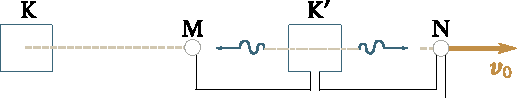
\includegraphics[scale=0.95]{figures/ch_08/fig_8_1.pdf}
		\caption[]{}
		\label{fig:8_1}
	\end{center}
\end{figure}

Trong hệ quy chiếu $K$ ánh sáng cũng truyền theo mọi hướng với vận tốc $c$. Trong hệ này vật $M$ chuyển động về phía tín hiệu sáng. Vật $N$ chuyển động cùng phía như tín hiệu.  Vì vậy tín hiệu đạt tới vật $M$ sớm hơn tới vật $N$, và do đó $t_{\text{M}}<t_{\text{N}}$. Như vậy, các biến cố đã xảy ra đồng thời trong hệ $K'$ sẽ xảy ra không đồng thời trong hệ $K$. Từ đó suy ra rằng thời gian trôi đi một cách không như nhau trong các hệ quy chiếu khác.

Để mô tả một biến cố trong một hệ quy chiếu nào đó, cần phải chỉ ra nó xảy ra ở chỗ nào và tại thời điểm nào. Vấn đề này là quan trọng nếu trong không gian thành lập các dấu tọa độ cách đều nhau và gắn với mỗi dấu như vậy một đồng hồ có thể xác định thời điểm biến cố xảy ra tại chỗ đã cho. Có thể vạch các dấu tọa độ bằng cách dời chỗ thang đơn vị. Để làm đồng hồ có thể lấy một hệ bất kỳ thực hiện một quá trình lặp lại một cách tuần hoàn. Để so sánh các thời điểm hai biến cô xảy ra tại các điểm khác nhau của không gian, cần phải tin tưởng rằng các đồng hồ nằm ở các điểm này chạy đồng bộ với nhau.

Hình như có thể thực hiện được sự đồng bộ hóa bằng cách, trước tiên đặt các đồng hồ thành một dãy và sau đó, sau khi kiểm lại sự chỉ của chúng người ta mang chúng tới các điểm tương ứng của không gian. Tuy vậy cần phải gạt bỏ biện pháp như thế, vì ta không biết sự vận chuyển của chúng từ chỗ này sang chỗ khác sẽ ảnh hưởng tới sự chuyển động của các đồng hồ như thế nào. Do đó trước tiên cần phải đặt các đồng hồ vào các chỗ và sau đó chỉ tiến hành sự kiểm tra lại sự chỉ của chúng. Điều này có thể làm được bằng cách gửi một tín hiệu sáng\footnote{Việc kiểm tra các đồng hồ theo các tín hiệu vô tuyến điện về bản chất là sự đồng bộ hóa như thế.} từ đồng hồ này sang đồng hồ khác. Giả thử từ một điểm $A$ tại thời điểm $t_1$ (được tính theo đồng hồ đặt tại A) người ta gửi đi một tín hiệu sáng được phản xạ từ một cái gương đặt tại điểm $B$ và trở lại $A$ tại thời điểm $t_2$. Cần phải coi đồng hồ ở $B$ là đồng bộ với đồng hồ ở $A$, nếu tại thời điểm mà tín hiệu trở về đến đồng hồ tại $A$ thì đồng hồ tại $B$ chỉ thời gian $t$ bằng $(t_1+t_2)/2$. Cần tiến hành sự kiểm lại như thế đối với tất cả các đồng hồ đặt tại các điểm khác nhau của hệ $K$. Các biến cố tại $A$ và $B$ sẽ được coi là đồng thời trong hệ $K$ nếu các sự tính thời gian tương ứng với chúng theo các đồng hồ $A$ và $B$ đều trùng nhau.

Người ta thực hiện một cách tương tự sự đồng bộ hóa tất cả các đồng hồ trong hệ $K'$ và trong mọi hệ quy chiếu quán tính khác. Vận tốc của tín hiệu sáng để thực hiện sự đồng bộ hóa là như nhau trong tất cả các hệ quy chiếu quán tính. Việc chọn làm tín hiệu cho sự đồng bộ hóa tiến trình của các đồng hồ, cụ thể là tín hiệu sáng, được quy định bằng chính điều đó. Thành ra vận tốc ánh sáng là vận tốc giới hạn. Không có một tín hiệu nào, không có một tác động nào của vật này lên vật kia có thể truyền với vận tốc vượt ánh sáng trong chân không. Sự đồng nhất của vận tốc ánh sáng trong chân không trong tất cả các hệ quán tính đều phải như nhau. Sự kiện là vận tốc của tín hiệu không thể vượt quá giá trị giới hạn cũng là một định luật của tự nhiên. Do đó giá trị của vận tốc giới hạn phải là như nhau trong tất cả hệ quy chiếu.

Sự bất biến của vận tốc ánh sáng dẫn tới điều là không gian và thời gian là liên quan lẫn nhau khi lập thành không-thời gian duy nhất. Mối liên hệ đó có thể được biểu diễn đặc biệt rõ ràng nhờ không gian bốn chiều tưởng tượng mà theo ba trục người ta đặt các tọa độ không gian $x$, $y$ và $z$, còn theo trục thứ 4, đó là thời gian $t$, chính xác hơn là tọa độ thời gian $ct$ tỷ lệ với $t$ có cùng thứ nguyên như các tọa độ không gian.

Một biến cố nào đó (chẳng hạn, sự phân rã của một hạt nào đó) được đặc trưng bởi chỗ, ở đó nó xẩy ra (bởi các tọa độ $x$, $y$, $z$) và bởi thời gian $t$, lúc nó xảy ra. Như vậy, điểm có các tọa độ $x$, $y$, $z$ và $ct$. trong không gian bốn chiều tưởng tượng ứng với biến cố này. Ta thường gọi điểm đó là \textit{điểm vũ trụ}. Một đường nào trong không gian bốn chiều tương ứng với mỗi hạt (ngay cả không chuyển động) được gọi là \textit{đường vũ trụ}. (đối với hạt đứng nghỉ nó có dạng đường thẳng song song với trục $ct$).

Như vậy, không gian và thời gian là các phần của một thể thống nhất. Tuy nhiên thời gian khác không gian về chất. Điều đó được thể hiện ở chỗ không gian bốn chiều tưởng tượng, về các tính chất của nó, khác khhông gian ba chiều thông thường. Không gian thông thường có metric Euclid. Điều đó có nghĩa là bình phương khoảng cách $\Delta l$ giữa hai điểm bằng tổng các bình phương các hiệu tọa độ:
\begin{equation*}
	\Delta l^2 = \Delta x^2 + \Delta y^2 + \Delta z^2.
\end{equation*}

Bình phương ``khoảng cách'' giữa hai điểm vũ trụ (``khoảng cách'' này được gọi là \textit{khoảng} và được ký hiệu bởi $\Delta s$) được xác định bởi công thức
\begin{equation}\label{eq:8_1}
	\Delta s^2 = c^2\Delta t^2 - \Delta x^2 - \Delta y^2 - \Delta z^2
\end{equation}

\noindent
(các tính chất của khoảng được xét trong Sec.~\ref{sec:8_4}).

Các không gian mà bình phương khoảng cách được xác định bởi công thức dạng~\eqref{eq:8_1} được gọi là các \textbf{không gian giả Euclid}. Sự khác nhau về chất giữa thời gian và không gian được thể hiện ở chỗ bình phương tọa độ thời gian và các bình phương các tọa độ không gian tham gia vào biểu thức \eqn{8_1} với các dấu khác nhau.

Các đại lượng là \textit{bất biến} đối với các phép biến đổi các tọa độ và thời gian từ hệ quy chiếu quán tính này sang hệ quy chiếu quán tính khác (nói cách khác, các đại lượng có trị số như nhau trong tất cả các hệ quy chiếu quán tính) đóng vai trò đặc biệt quan trọng trong thuyết tương đối hẹp. Ta đã biết một trong các đại lượng như vậy --- đó là vận tốc ánh sáng trong chân không. Trong Sec.~\ref{sec:8_4} ta chứng tỏ rằng khoảng được xác định bởi công thức \eqn{8_1} cùng là một bất biến.

Các công thức và các hệ thức bất biến đối với các phép biến đổi đã nói ở trên (tức là có cùng dạng trong tất cả các hệ quy chiếu quán tính) cũng đóng vai trò đặc biệt quan trọng. Chẳng hạn, các biểu thức tương đối tính đối với xung lượng và năng lượng được xác định bằng cách sao cho các định luật bảo toàn của các đại lượng này không bị vi phạm khi chuyển sang hệ quy chiếu quán tính khác. Trong tiến trình được trình bày sau đây chúng ta sẽ làm quen với một loạt đại lượng và hệ thức bất biến.

\section{Các biến đổi Lorentz}\label{sec:8_2}

Ta xét hai hệ quy chiếu quán tính mà ta ký hiệu là $K$ và $K'$ (hình \fig{8_2}). Giả sử hệ $K'$ chuyển động đối với hệ $K$ với vận tốc $\vec{v}_0$\footnote{Ta nhớ rằng hệ quy chiếu quán tính là hệ quy chiếu mà đối với nó một hạt tự do sẽ chuyển động không có gia tốc (xem Sec.~\ref{sec:2_2}). Trong Sec.~\ref{sec:2_7} dựa vào các phép biến đổi Galileo ta đã chứng tỏ rằng một hệ $K'$ chuyển động đối với hệ quán tính $K$ với vận tốc không đổi $\vec{v}_0$, thì đến lượt mình $K'$ là hệ quán tính. Trong cơ học tương đối tính các phép biến đổi Galileo phải được thay bởi các phép biến đổi khác tuân theo nguyên lý bất biến của vận tốc ánh sáng. Tuy nhiên rõ ràng rằng dù định luật biến đổi, khi chuyển từ hệ $K$ sang hệ $K'$ chuyển động đối với $K$ với vận tốc không đổi $\vec{v}_0$, có là thế nào đi nữa thì khi nào vận tốc $\vec{v}$ của hạt trong hệ $K$ là không đổi $\vec{v}_0$, có là thế nào đi nữa thì khi nào vận tốc $\vec{v}$ của hạt trong hệ $K$ là không đổi, vận tốc $\vec{v}'$ cũng sẽ không đổi trong hệ $K'$. Do đó, cả trong cơ học tương đối tính hệ $K'$ chuyển động đối với hệ quán tính $K$ với vận tốc không đổi $\vec{v}_0$ cũng sẽ là hệ quán tính.}. Ta hướng các trục $x$ và $x'$ dọc theo vector $\vec{v}_0$ và giả thiết các trục $y$ và $y'$ cũng như $z$ và $z'$ là song song với nhau.

\begin{figure}[!htb]
	\begin{center}
		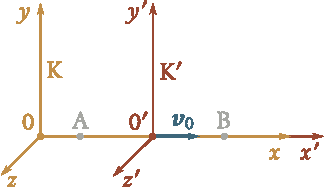
\includegraphics[scale=0.95]{figures/ch_08/fig_8_2.pdf}
		\caption[]{}
		\label{fig:8_2}
	\end{center}
\end{figure}

Theo nguyên lý tương đối các hệ $K$ và $K'$ là hoàn toàn bình đẳng. Sự khác nhau về hình thức duy nhất của chúng là ở chỗ tọa độ theo trục $x$ của gốc $O'$ của hệ $K'$ được tính trong hệ $K$ sẽ biến thiên theo quy luật
\begin{equation}\label{eq:8_2}
	x_{0}' = v_0 t
\end{equation}

\noindent
trong khi tọa độ theo trục $x$ của gốc $O$ của hệ $K$ được tính trong hệ $K'$ biến thiên theo quy luật
\begin{equation}\label{eq:8_3}
	x_0' = - v_0 t'.
\end{equation}

\noindent
Sự khác nhau này được gây ra bởi điều là ta đã chọn các hướng của các trục $x$ và $x'$ là như nhau, còn các hệ $K$ và $K'$ chuyển động đối với nhau theo các hướng ngược nhau. Vì vậy, hình chiếu của vận tốc tương đối lên trục $x$ của hệ $K$ bằng $\vec{v}_0$, còn lên trục $x'$ của hệ $K'$ bằng $-\vec{v}_0$.

Trong cơ học phi tương đối tính việc chuyển từ các tọa độ và thời gian của hệ quy chiếu quán tính này sang các tọa độ và thời gian của hệ quán tính khác được thực hiện nhờ các phép biến đổi Galileo~\eqref{eq:2_9}. Từ các phép biến đổi này suy ra định luật cộng các vận tốc: $\vec{v}=\vec{v}'+\vec{v}_0$ (xem công thức \eqn{2_21}). Định luật này mâu thuẫn với nguyên lý bất biến của vận tốc ánh sáng. Thực vậy, nếu trong hệ $K'$ tín hiệu sáng truyền theo hướng của vector $\vec{v}_0$ với vận tốc $c$, thì theo \eqn{2_21} trong hệ $K$ vận tốc của tín hiệu là bằng $c+v_0$, tức là vượt quá $c$. Từ đó suy ra rằng các phép biến đổi Galileo phải được thay bởi các công thức khác. Dễ dàng tìm được các công thức này.

Dưới dạng tổng quát nhất các phép biến đổi các tọa độ và thời gian từ hệ $K'$ sang hệ $K$ thể hiện như sau:
\begin{equation}\label{eq:8_4}
	\begin{cases}
		&\!\!\!\! x = f_1(x',y',z',t'),\quad y = f_2(x',y',z',t'),\\
		&\!\!\!\! z = f_3(x',y',z',t'),\quad t = f_4(x',y',z',t').
	\end{cases}
\end{equation}

\noindent
Từ tính đồng tính của thời gian và không gian suy ra rằng các công thức Eqs.~\eqref{eq:8_4} phải là tuyến tính, tức là có dạng
\begin{equation}\label{eq:8_5}
	x = \alpha_1 x' + \alpha_2 y' + \alpha_3 z' + \alpha_4 t' + \alpha_5
\end{equation}

\noindent
và v.v$\ldots$, trong đó $\alpha_1, \alpha_2, \ldots$ là các hằng số. Một cách tương ứng
\begin{equation}\label{eq:8_6}
	\deriv{x} = \alpha_1\,\deriv{x'} + \alpha_2\,\deriv{y'} + \alpha_3\,\deriv{z'} + \alpha_4\,\deriv{t'}
\end{equation}

\noindent
và v.v$\ldots$.

Thực vậy, theo Eqs.~\eqref{eq:8_4}
\begin{align}
	\deriv{x} &= \diffpartial{f_1}{x'}\deriv{x'} + \diffpartial{f_2}{y'}\deriv{y'} + \diffpartial{f_3}{z'}\deriv{z'} + \diffpartial{f_4}{t'}\deriv{t'}\label{eq:8_7}\\
	&\vdots\quad\quad\vdots\quad\quad\vdots\quad\quad\vdots\quad\quad\vdots\quad\quad\vdots\quad\quad\vdots\nonumber
\end{align}

\noindent
Nếu lấy $\deriv{x'}, \deriv{y'}, \deriv{z'}$ và $\deriv{t'}$ được chọn một cách tùy ý tại điểm $x_1', y_1', z_1', t_1'$ thì khi thế các giá trị của các đạo hàm tại điểm đã cho vào Eqs.~\eqref{eq:8_7} ta được giá trị $\deriv{x_1}$ nào đó của $\deriv{x}$. Tuy nhiên, do tính đồng tính của không gian và thời gian tại một điểm bất kỳ nào khác $x_2', y_2', z_2', t_2'$ với cùng các giá trị $\deriv{x'}, \deriv{y'}, \deriv{z'}$ và $\deriv{t'}$ phải thu được cùng giá trị của $\deriv{x}$ như tại điểm thứ nhất, tức là phải có $\deriv{x_2}=\deriv{x_1}$. Cũng hệt như vậy, phải xảy ra đối với $\deriv{y}, \deriv{z}$ và $\deriv{t}$. Vì $\deriv{x'}, \deriv{y'}, \deriv{z'}$ và $\deriv{t'}$ được chọn hoàn toàn tùy ý nên đòi hỏi đã nêu chỉ có thể được thực hiện trong trường hợp nếu các đạo hàm $\diffpartial{f_1}{x'}$, v.v$\ldots$ không phụ thuộc vào các tọa độ, tức là vào các hằng số. Từ đó suy ra \eqn{8_6} và sau đó cả \eqn{8_5}.

Với việc chọn các trục tọa độ đã chỉ trên hình \fig{8_2} mặt phẳng $y=0$ trùng với mặt phẳng $y'=0$, còn mặt phẳng $z=0$ trùng với mặt phẳng $z'=0$. Từ đó suy ra rằng, chẳng hạn, các tọa độ $y$ và $y'$ phải triệt tiêu đồng thời, độc lập với các giá trị của các tọa độ khác và của thời gian. Vì vậy $y$ và $y'$ chỉ có thể được liên hệ với nhau bởi hệ thức dạng
\begin{equation*}
	y = \varepsilon y'
\end{equation*}

\noindent
trong đó $\varepsilon$ là một hằng số. Do tính bình đẳng của các hệ $K$ và $K'$ nên hệ thức ngược phải có dạng
\begin{equation*}
	y' = \varepsilon y
\end{equation*}

\noindent
với cùng giá trị của hằng số $\varepsilon$ Như trong trường hợp thứ nhất. Nhân cả hai hệ thức với nhau ta được $\varepsilon^2 = 1$, từ đó $\varepsilon=\pm 1$. Dấu cộng ứng với các trục $y$ và $y'$ cùng chiều, dấu trừ --- ngược chiều. Khi các trục cùng chiều ta có
\begin{equation}\label{eq:8_8}
	y = y'.
\end{equation}

\noindent
Các lập luận tương tự dẫn tới công thức
\begin{equation}\label{eq:8_9}
	z = z'.
\end{equation}

Ta chuyển sang tìm các phép biến đổi đối với $x$ và $t$. Từ Eqs.~\eqref{eq:8_8} và~\eqref{eq:8_9} suy ra rằng các giá trị $y$ và $z$ không thể phụ thuộc vào $x'$ và $t'$. Từ đó suy ra rằng các giá trị $x'$ và $t'$ không thể phụ thuộc vào $y$ và $z$; một cách tương ứng các giá trị $X$ và $t$ không thể phụ thuộc vào $y'$ và $z'$. Như vậy, $x$ và $t$ có thể là những hàm tuyến tính chỉ của $x'$ và $t'$.

Gốc tọa độ $O$ của hệ $K$ có tọa độ $x=0$ trong hệ $K$ và $x'=-v_0 t'$ trong hệ $K'$ [see \eqn{8_3}]. Do đó biểu thức $(x'+v_0 t')$ phải triệt tiêu đồng thời với tọa độ $x$. Muốn thế phép biến đổi tuyến tính phải có dạng
\begin{equation}\label{eq:8_10}
	x = \gamma (x' + v_0 t')
\end{equation}

\noindent
trong đó $\gamma$ là một hằng số nào đó.

Tương tự, gốc tọa độ $O'$ của hệ $K'$ có tọa độ $x'=0$ trong hệ $K'$ và $x=v_0 t$ trong hệ $K$ [see \eqn{8_2}]. Từ đó suy ra rằng
\begin{equation}\label{eq:8_11}
	x' = \gamma (x - v_0 t)
\end{equation}

\noindent
Từ sự bình đẳng của các hệ $K$ và $K'$ suy ra rằng hệ số tỷ lệ trong cả hai trường hợp phải là như nhau.

Để tìm hệ số $\omega$ ta sử dụng nguyên lí bất biến của vận tốc ánh sáng. Ta bắt đầu tính thời gian trong cả hai hệ từ thời điểm khi các gốc tọa độ của chúng trùng nhau. Giả sử tại thời điểm $t=t'=0$ theo hướng của các trục $x$ và $x'$ tín hiệu sáng được gửi đi tạo ra tia chớp sáng trên tấm chắn đặt tại điểm có tọa độ $x$ trong hệ $K$ và tọa độ $x'$ trong hệ $K'$. Sự kiện này (chớp sáng) được mô tả bởi tọa độ $x$ và thời điểm $t$ trong hệ $K$ và bởi tọa độ $x'$ và thời điểm $t'$ trong hệ $K'$, hơn nữa
\begin{equation*}
	x = ct,\quad x' = ct'.
\end{equation*}

\noindent
Thế các giá trị của $x$ và $x'$ vào các công thức Eqs.~\eqref{eq:8_10} và~\eqref{eq:8_11} ta được
\begin{align*}
	ct  &= \gamma (ct' + v_0 t') = \gamma (c + v_0)t',\\
	ct' &= \gamma (ct - v_0 t) = \gamma (c - v_0)t.
\end{align*}

Nhân cả hai hệ thức với nhau, ta đi tới phương trình
\begin{equation}\label{eq:8_12}
	\gamma = \frac{1}{\left[1 - \left(v_0^2/c^2\right)\right]^{1/2}}.
\end{equation}

\noindent
Phép thế giá trị này vào \eqn{8_10} sẽ dẫn tới công thức
\begin{equation}\label{eq:8_13}
	x = \frac{x + v_0 t'}{\left[1 - \left(v_0^2/c^2\right)\right]^{1/2}}.
\end{equation}

Công thức~\eqref{eq:8_13} cho phép tìm giá trị $x$ theo các giá trị đã biết $x'$ và $t'$. Để nhận được công thức cho phép tìm giá trị $t$ theo các giá trị đã biết $x'$ và $t'$, ta khử các tọa độ $x$ từ Eqs.~\eqref{eq:8_10} và~\eqref{eq:8_11} và giải hệ thức nhận được đối với $t$. Kết quả là ta có
\begin{equation*}
	t = \gamma \left[t' + \frac{x'}{v_0}\left(1 - \frac{1}{\gamma^2}\right)\right].
\end{equation*}

\noindent
Phép thế giá trị \eqn{8_12} đối với $\gamma$ dẫn tới công thức sau:
\begin{equation}\label{eq:8_14}
	t = \frac{t' + (v_0/c^2) x'}{\left[1 - \left(v_0^2/c^2\right)\right]^{1/2}}.
\end{equation}

Tập hợp các công thức Eqs.~\eqref{eq:8_8}, \eqref{eq:8_9}, \eqref{eq:8_13}, và~\eqref{eq:8_14} mang tên các \textbf{phép biến đổi Lorentz}. Nếu sử dụng ký hiệu phổ biến
\begin{equation}\label{eq:8_15}
	\beta = \frac{v_0}{c}
\end{equation}

\noindent
thì các phép biến đổi Lorentz có dạng
\begin{equation}\label{eq:8_16}
	x = \frac{x + \beta ct'}{\left(1 - \beta^2\right)^{1/2}},\quad y = y',\quad z = z',\quad t = \frac{t' + (\beta/c) x'}{\left(1 - \beta^2\right)^{1/2}}.
\end{equation}

Việc chuyển từ các tọa độ và thời gian được tính trong hệ $K'$ sang các tọa độ và thời gian được tính trong hệ $K'$ (một cách ngắn gọn, việc chuyển từ hệ $K'$ sang hệ $K$) được thực hiện theo các công thức~\eqref{eq:8_16}. Nếu giải các phương trình Eqs.~\eqref{eq:8_16}  đối với các đại lượng có dấu phẩy, sẽ thu được các công thức biến đổi để chuyển từ hệ $K$ sang hệ $K'$:
\begin{equation}\label{eq:8_17}
	x' = \frac{x - \beta ct}{\left(1 - \beta^2\right)^{1/2}},\quad y' = y,\quad z' = z,\quad t' = \frac{t - (\beta/c) x}{\left(1 - \beta^2\right)^{1/2}}.
\end{equation}

Cũng như điều cần mong chờ, nếu để ý tới tính bình đẳng của các hệ $K$ và $K'$, các công thức Eqs.~\eqref{eq:8_17} chỉ khác các công thức~\eqref{eq:8_16} bởi dấu trước $\beta$, tức là trước $v_0$.

Dễ dàng hiểu rằng trong trường hợp $v_0\ll c$ (tức là $\beta\ll 1$) các phép biến đổi Lorentz chuyển thành các phép biến đổi Galileo [xem Eqs.~\eqref{eq:2_19}]. Như vậy, các phép biến đổi Galileo vẫn bảo toàn giá trị đối với vận tốc nhỏ so với vận tốc ánh sáng trong chân không.

Khi $v_0>c$ các biểu thức Eqs.~\eqref{eq:8_16} và~\eqref{eq:8_17} đối với $x$, $t$, $x'$, và $t'$ trở thành ảo. Điều này phù hợp với điều là chuyển động với vận tốc vượt quá vận tốc ánh sáng trong chân không là không thể xảy ra. Không được sử dụng ngay cả hệ quy chiếu chuyển động với vận tốc $c$, vì khi $v_0=c$ ở các mẫu số trong các công thức đối với $x$ và $t$ sẽ bằng số không.

Các phép biến đổi Lorentz có dạng đặc biệt đơn giản và đối xứng nếu viết chúng không phải đối với $x$ và $t$ mà đối với $x$ và $(ct)$, tức là đối với các đại lượng có cùng thứ nguyên. Trong trường hợp đó các công thức~\eqref{eq:8_16} thể hiện như sau:
\begin{equation}\label{eq:8_18}
	x = \frac{x' + \beta (ct)'}{\left(1 - \beta^2\right)^{1/2}},\quad y = y',\quad z = z',\quad t = \frac{(ct)' + \beta x'}{\left(1 - \beta^2\right)^{1/2}}.
\end{equation}

Dễ dàng nhớ được các công thức Eqs.~\eqref{eq:8_18} bằng cách chú ý rằng công thức thứ nhất trong chúng khác công thức ``hiển nhiên'' $x=x'+v_0t'$ bởi sự có mặt ở mẫu số biểu thức $\left(1 - \beta^2\right)^{1/2}$ đặc trưng cho các công thức tương đối tính. Công thức cuối nhận được từ công thức thứ nhất nếu hoán vị các vị trí của $x'$ và $ct'$.

\section{Các hệ quả của các biến đổi Lorentz}\label{sec:8_3}

Từ các biến đổi Lorentz suy ra một loạt kết luận khác thường so với quan điểm của cơ học Newton.

\textbf{Tính đồng thời của các biến cố trong các hệ quy chiếu khác nhau.} Giả sử trong hệ quy chiếu $K$ tại các điểm có các tọa độ $x_1$ và $x_2$ xảy ra đồng thời hai biến cố tại thời điểm $t=1=t=2=b$. Theo công thức cuối trong~\eqref{eq:8_17} trong hệ $K'$ các biến cố này sẽ ứng với các thời điểm
\begin{equation*}
	t_1' = \frac{b - (\beta/c) x_1}{\left(1 - \beta^2\right)^{1/2}},\quad t_2' = \frac{b - (\beta/c) x_2}{\left(1 - \beta^2\right)^{1/2}}
\end{equation*}

\noindent
Từ các công thức này rõ ràng trong trường hợp nếu trong hệ $K$ các biến cố biệt lập về không gian $(x_1\neq x_2)$ thì trong hệ $K'$ chúng sẽ không xảy ra đồng thời $(t_1'\neq t_2')$. Dấu của hiệu $t_2'-t_1'$ được xác định bởi dấu của biểu thức $(\beta/c)(x_1-x_2)$; do đó trong các hệ $K'$ khác nhau (với các $\beta$ khác nhau) hiệu $t_2'-t_1'$ sẽ khác nhau về độ lớn và có thể được phân biệt về dấu. Điều này có nghĩa là trong các hệ này biến cố $1$ sẽ xảy ra trước biến cố $2$, ngược lại trong các hệ khác biến cố $2$ sẽ xảy ra trước biến cố $1$. Ta chú ý rằng điều đã nói chỉ liên quan tới các biến cố mà giữa chúng không có quan hệ nhân quả. Các biến cố có quan hệ nhân quả (chẳng hạn, sự ném hòn đá và sự rơi của nó xuống đất) sẽ không xảy ra đồng thời trong một hệ quy chiếu nào, và trong mọi hệ biến cố là nguyên nhân sẽ xảy ra trước kết quả. Chi tiết hơn về điều này sẽ nói ở mục sau.

\begin{figure}[!htb]
	\begin{center}
		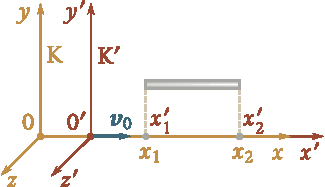
\includegraphics[scale=0.95]{figures/ch_08/fig_8_3.pdf}
		\caption[]{}
		\label{fig:8_3}
	\end{center}
\end{figure}

\textbf{Độ dài của các vật trong các hệ khác nhau.} Ta xét một thanh được đặt dọc theo trục $x'$ và đứng yên đối với hệ quy chiếu $K'$ (\fig{8_3}). Độ dài của nó trong hệ này là bằng $l_0=x_2'-x_1'$, trong đó $x_1'$ và $x_2'$ là các tọa độ của các đầu mút của thanh không biến đổi với thời gian $t'$. Đối với hệ $K$ thanh chuyển động với vận tốc $v=v_0$. Để xác định độ dài của nó trong hệ này cần đánh dấu các tọa độ $x_1$ và $x_2$ của các đầu mút của thanh tại cùng một thời điểm $t_1=t_2=b$. Hiệu $l=x_2-x-1$ của chúng cho độ dài của thanh được đo trong hệ $K$. Để tìm hệ thức giữa $l_0$ và $l$ cần phải lấy một trong các công thức biến đổi Lorentz có chứa $x'$, $x$ và $t$, nghĩa là công thức thứ nhất trong các công thức~\eqref{eq:8_17}. Trong công thức này thay $\beta$ bằng $v_0/c$, ta có:
\begin{equation*}
	x_1' = \frac{x_1 - v_0 b}{\left[1 - \left(v_0^2/c^2\right)\right]^{1/2}},\quad x_2' = \frac{x_2 - v_0 b}{\left[1 - \left(v_0^2/c^2\right)\right]^{1/2}}
\end{equation*}

\noindent
từ đó
\begin{equation*}
	x_2' - x_1' = \frac{x_2 - x_1}{\left[1 - \left(v_0^2/c^2\right)\right]^{1/2}}.
\end{equation*}

\noindent
Sử dụng các ký hiệu $l$ và $l_0$, cũng như thay vận tốc tương đối của các hệ quy chiếu $v_0$ bằng vận tốc $v$ của thanh đối với hệ $K$ (mà $v=v_0$) ta sẽ đi tới hệ thức
\begin{equation}\label{eq:8_19}
	l = l_0 \left(1 - \frac{v_0^2}{c^2}\right)^{1/2}.
\end{equation}

\noindent
Như vậy, độ dài $l$ của thanh được đo trong hệ mà thanh chuyển động đối với nó sẽ nhỏ hơn độ dài $l_0$ được đo trong hệ mà thanh đứng yên\footnote{Đôi khi người ta gọi độ dài $l_0$ được đo trong hệ mà thanh đứng yên đối với nó là \textbf{độ dài riêng} của thanh.} đối với nó.

Nếu thanh có độ dài $l_0=x_2-x_1$ đứng yên đối với hệ $K$, thì để xác định độ dài của nó trong hệ $K'$ cần phải đánh dấu các tọa độ $x_1'$ và $x_2'$ của các đầu mút tại cùng một thời điểm $t_1'=t_2'=b$. Hiệu $l=x_2'-x_1'$ cho độ dài của thanh trong hệ $K'$ mà thanh chuyển động với vận tốc $v$ đối với nó. Sử dụng phương trình thứ nhất trong các phương trình~\eqref{eq:8_16} ta lại đi tới hệ thức \eqn{8_19}.

Ta chú ý rằng các kích thước của thanh theo các phương của các trục $y$ và $z$ đều như nhau trong tất cả các hệ quy chiếu.

Như vậy, ở các vật chuyển động vận tốc chuyển động càng lớn chừng nào thì các kích thước theo phương chuyển động của chúng càng bị co lại chừng ấy. Hiện tượng này được gọi là \textbf{sự co Lorentz} (hoặc \textbf{sự co Fitzgerald}). Đáng chú ý là sự thay đổi có thể nhìn bằng mắt thường (hoặc trên bức ảnh chụp) về hình dạng của vật, ngay cả với các vận tốc có thể so sánh được với $c$, cũng không thể phát hiện được. Nguyên nhân của điều này là rất đơn giản. Khí quan sát bằng mắt thường hoặc khi chụp ảnh một vật nào đó ta ghi được các xung lượng ánh sáng từ các phần khác nhau của vật đồng thời đạt tới võng mạc của mắt hoặc tới phim ảnh. Chính các xung đó được phát ra đồng thời. Các xung từ các phần xa hơn được phát ra sớm hơn so với các xung từ các phần gần hơn. Như vậy, nếu vật chuyển động thì trên võng mạc của mắt hoặc trên bức ảnh chụp ta thu được hình ảnh sai lạc của vật. Sự tính toán thích hợp chứng tỏ rằng kết quả của sự sai lạc đã nêu sẽ bù trừ cho sự co Lorentz\footnote{Nếu không có sự co Lorentz thì vật chuyển động nhanh phải được kéo dài theo phương chuyển động.}, cho nên các vật hầu như không bị méo mó mà chỉ bị quay đi. Do đó một vật có dạng hình cầu ngay khi chuyển động với các vận tốc lớn cũng sẽ được lĩnh hội bằng mắt thường là một vật có dạng hình cầu.

\textbf{Khoảng thời gian giữa các biến cố.} Giả sử tại cùng một điểm của hệ $K'$ xảy ra hai biến cố. Trong hệ đó biến cố thứ nhất ứng với tọa độ $x_1'=a$ và thời điểm $t_1'$, biến cố thứ hai --- tọa độ $x_2'=a$ và thời điểm $t_2'$. Theo công thức cuối trong các công thức~\eqref{eq:8_16} trong hệ $K$ các biến cố này ứng với các thời điểm
\begin{equation*}
	t_1 = \frac{t_1' + (v_0/c)^2 a}{\left[1 - \left(v_0^2/c^2\right)\right]^{1/2}},\quad t_2 = \frac{t_2' + (v_0/c^2) a}{\left[1 - \left(v_0^2/c^2\right)\right]^{1/2}}.
\end{equation*}

\noindent
(ta đã thay $\beta$ bằng $v_0/c$). Từ đó
\begin{equation*}
	t_2 - t_1 = \frac{t_2' - t_2'}{\left[1 - \left(v_0^2/c^2\right)\right]^{1/2}}.
\end{equation*}

Đưa vào các ký hiệu $t_2-t_1=\Delta t$ và $t_2'-t_1'=\Delta t'$, ta có được công thức
\begin{equation}\label{eq:8_20}
	\Delta t = \frac{\Delta t'}{\left[1 - \left(v_0^2/c^2\right)\right]^{1/2}}
\end{equation}

\noindent
liên hệ các khoảng thời gian giữa hai biến cố được đo trong các hệ $K$ và $K'$. Ta nhớ rằng trong hệ $K'$ cả hai biến cố xảy ra tại cùng một điểm $x_1=x_2'$.

Giả sử cả hai biến cố xuất phát từ cùng một hạt đứng yên trong hệ $K'$ và chuyển động đối với hệ $K$ với vận tốc $v=v_0$. Khi đó có thể giải thích $\Delta t'$ như khoảng thời gian được đo theo đồng hồ không chuyển động đối với hạt hoặc, nói cách khác, được đo theo đồng hồ chuyển động cùng với hạt (khi lưu ý tới sự chuyển động đối với hệ $K$). Thời gian được tính theo đồng hồ chuyển động cùng với vật được gọi là \textbf{thời gian riêng} của vật đó và thường được ký hiệu bằng chữ $\tau$. Như vậy, $\Delta t'=\Delta\tau$. Để ý đến điều này, công thức \eqn{8_20} có thể nhận dạng
\begin{equation}\label{eq:8_21}
	\Delta\tau = \Delta t \left[1 - \left(v^2/c^2\right) \right]^{1/2}
\end{equation}

\noindent
(ta đã thay vận tốc tương đối $v_0$ của các hệ quy chiếu bằng vận tốc $v$ của hạt).

Công thức~\eqref{eq:8_21} liên hệ thời gian riêng $\tau$ của vật với thời gian $t$ được tính theo đồng hồ của hệ quy chiếu mà vật chuyển động với vận tốc $v$ đối với nó (chính đồng hồ này chuyển động đối với vật với vận tốc $-v$).

Từ \eqn{8_21}, luôn luôn bé hơn thời gian được tính theo đồng hồ chuyển động đối với vật. Trong mục sau chúng ta chứng tỏ rằng thời gian riêng là bất biến (tức là như nhau trong tất cả các hệ quy chiếu).

Khi xét các biến cố xảy ra cùng với hạt trong hệ $K$ có thể xác định $\Delta t$ như khoảng thời gian đo theo đồng hồ không chuyển động, còn $\Delta\tau$ --- như khoảng thời gian đo theo đồng hồ chuyển động với vận tốc $v$. Theo \eqn{8_21} $\Delta\tau<\Delta t$; vì vật có thể nói rằng đồng hồ chuyển động chạy chậm hơn đồng hồ đứng yên (chú ý rằng, ngoài vận tốc chuyển động, các đồng hồ đều hoàn toàn như nhau về mọi phương diên).

Hệ thức~\eqref{eq:8_21} đã được xác nhận bằng thực nghiệm một cách trực tiếp. Trong thành phần của các tia vũ trụ có các hạt $\mu$---meson hoặc muon. Các hạt này không bền, nghĩa là chúng tự phân rã thành một electron (hoặc positron) và hai neutrino. Thời gian sống trung bình được đo trong các điều kiện khi chúng đứng nghỉ (hoặc chuyển động với vận tốc nhỏ) là vào khoảng \SI{2e-6}{\second}. Nhưng hình như là ngay cả khi chuyển động với vận tốc ánh sáng các meson cũng chỉ có thể đi được một quãng đường vào cỡ \SI{600}{\metre}. Tuy nhiên như các quan sát chứng tỏ các meson được tạo thành trong các tia vũ trụ ở độ cao \SIrange{20}{30}{\kilo\metre} và đi đến mặt đất với một lượng đáng kể. Điều này được giải thích bởi điều là \SI{2e-6}{\second} là thời gian sống riêng của meson, tức là thời gian được đo theo đồng hồ chuyển động cùng với nó. Thời gian được tính theo đồng hồ của một nhà thực nghiệm gắn với Trái đất sẽ lớn hơn nhiều [xem \eqn{8_21}; $v$ của meson gần với $c$]. Vì vậy không có gì đáng ngạc nhiên về việc nhà thực nghiệm này quan sát được quãng đường đi của meson lớn hơn \SI{600}{\metre} một cách đáng kể. Ta chú ý rằng theo quan điểm của người quan sát chuyển động cùng với meson, khoảng cách do các meson, bay được tới mặt đất bị rút ngắn đến \SI{600}{\metre} [xem \eqn{8_19}], cho nên meson bay được khoảng cách này trong \SI{2e-6}{\second}.

\section{Khoảng}\label{sec:8_4}

Trong Sec.~\ref{sec:8_1} đã nói rằng mỗi biến cố này có tọa độ $ct_1$, $x_1$, $y_1$, $z_1$ biến cố khác có tọa độ $ct_2$, $x_2$, $y_2$, $z_2$. Ta đưa vào các ký hiệu $t_2-t_1=\Delta t$, $x_2-x_1=\Delta x$ v.v \ldots

Ta nhớ rằng, do sự khác nhau về chất giữa thời gian và không gian, nên bình phương của hiệu các tọa độ thời gian $(c\Delta t)^2$ và các bình phương của hiệu các tọa độ không gian $\Delta x^2$, $\Delta y^2$, $\Delta z^2$ tham gia vào biểu thức đối với bình phương ``khoảng cách'' giữa các biến cố (chính xác hơn, giữa các điểm vũ trụ ứng với các biến cố) với các dấu khác nhau:
\begin{equation}\label{eq:8_22}
	\Delta s^2 = c^2\Delta t^2 - \Delta x^2 - \Delta y^2 - \Delta z^2.
\end{equation}

\noindent
Đại lượng $\Delta s$ được xác định bởi công thức này được gọi là \textbf{khoảng} giữa các biến cố.

Nếu đưa vào các khoảng cách $\Delta l=\left(\Delta x^2+\Delta y^2+\Delta z^2\right)^{1/2}$ giữa các điểm của không gian ba chiều thông thường, trong đó các biến cố đang xét đã xảy ra, thì có thể biểu diễn biểu thức đối với khoảng dưới dạng
\begin{equation}\label{eq:8_23}
	\Delta s = \left(c^2\Delta t^2 - \Delta l^2\right)^{1/2}.
\end{equation}

Dễ dàng thấy rằng khoảng giữa hai biến cố đã cho trong tất cả các hệ quy chiếu quán tính là như nhau. Chính điều đó là cơ sở vững chắc để xem nó là một tương tự của khoảng cách $\Delta l$ giữa hai điểm trong không gian ba chiều thông thường ($\Delta l$ không thay đổi giá trị của nó khi chuyển từ một hệ quy chiếu ba chiều này sang hệ quy chiếu ba chiều khác).

Giả sử có hệ quy chiếu $K$, bình phương của khoảng được xác định bởi công thứ \eqn{8_22}. Bình phương của khoảng giữa cũng các biến cố đó trong hệ $K'$ bằng
\begin{equation}\label{eq:8_24}
	\Delta s'^2 = c^2\Delta t'^2 - \Delta x'^2 - \Delta y'^2 - \Delta z'^2.
\end{equation}

\noindent
Theo các công thức Eqs.~\eqref{eq:8_17}
\begin{equation*}
	\Delta x' = \frac{\Delta x - \beta c\Delta t}{\left(1 - \beta^2\right)^{1/2}},\quad \Delta y' = \Delta y,\quad \Delta z' = \Delta z,\quad 	\Delta t' = \frac{\Delta t - (\beta/c)\Delta x}{\left(1 - \beta^2\right)^{1/2}}.
\end{equation*}

\noindent
Thế các giá trị này vào công thức \eqn{8_24}, sau các biến đổi đơn giản ta được $\Delta s'^2 = c^2\Delta t^2 - \Delta x^2 - \Delta y^2 - \Delta z^2$, tức là
\begin{equation*}
	\Delta s'^2 = \Delta s^2.
\end{equation*}

Như vậy, khoảng là một bất biến đối với sự chuyển từ hệ quy chiếu quán tính này sang hệ quy chiếu quán tính khác. Trong mục trước ta đã thấy rằng các khoảng thời gian $\Delta t$ và các độ dài $\Delta l$ đối với sự chuyển như thế không phải là các bất biến. Do đó, mỗi số hạng tạo thành đại lượng $\Delta s^2=c^2\Delta t^2-\Delta t^2$ bị biến đổi khi chuyển từ hệ này sang hệ khác; còn chính đại lượng $\Delta s^2$ lại không đổi.

Khoảng giữa hai biến cố xuất phát từ một hạt nào đó tỷ lệ đơn giản với khoảng thời gian riêng giữa các biến cố đó. Theo \eqn{8_21} khoảng thời gian riêng $\Delta \tau^2$ sẽ liên hệ với khoảng thời gian $\Delta t$, được tính theo đồng hồ của hệ mà hạt chuyển động với vận tốc $v$ đối với nó, bởi công thức
\begin{equation*}
	\Delta\tau = \Delta t\left(1 - \frac{v^2}{c^2}\right).
\end{equation*}

\noindent
Ta biến đổi công thức này như sau:
\begin{equation*}
	\Delta\tau = \frac{1}{c}\left[c^2\Delta t^2 - (v\Delta t)^2\right]^{1/2} = \frac{1}{c}\left(c^2\Delta t^2 - \Delta l^2\right)^{1/2}.
\end{equation*}

\noindent
Ở đây $\Delta l=v\Delta t$ là quãng đường do hạt đi được trong khoảng thời gian $\Delta t$. So sánh với \eqn{8_23} cho
\begin{equation}\label{eq:8_25}
	\Delta\tau = \frac{1}{c}\Delta s
\end{equation}

\noindent
trong đó $\Delta s$ là khoảng giữa các biến cố được tách bởi khoảng thời gian $\Delta\tau$.

Từ công thức \eqn{8_25} suy ra rằng khoảng thời gian riêng tỷ lệ với khoảng giữa các biến cố. Khoảng là một bất biến. Do đó, thời gian riêng là một bất biến, tức là không phụ thuộc vào sự chuyển động của vật đã cho được quan sát trong hệ quy chiếu nào.

Theo công thức \eqn{8_23} khoảng có thể là thực (nếu $c\Delta t>\Delta l$) hoặc ảo (nếu $c\Delta t<\Delta l$), trong trường hợp riêng khoảng có thể bằng không (nếu $c\Delta t=\Delta l$). Trường hợp cuối xảy ra đối với các biến cố là sự phát tín hiệu sáng từ điểm $x_1, y_1, z_1$ tại thời điểm $t_1$ và sự chuyển tín hiệu đó vào điểm $x_2, y_2, z_2$ tại thời điểm $t_2$. Bởi vì trong trường hợp đó $\Delta l=c\Delta t$ nên khoảng giữa các biến cố bằng không.

Do tính bất biến nên khoảng là thực (ảo) trong một hệ quy chiếu $K$ nào đó sẽ là thực (ảo) trong một hệ quán tính $K'$ bất kỳ khác.

Trong trường hợp khoảng thực
\begin{equation*}
	c^2\Delta t^2 - \Delta l^2 = c^2\Delta t^2 - \Delta l'^2 > 0.
\end{equation*}

\noindent
Từ hệ thức này suy ra rằng có thể tìm được một hệ $K'$ trong đó $\Delta l'=0$, tức là cả hai biến cố chồng lên nhau về không gian. Tuy nhiên không tồn tại một hệ quy chiếu trong đó đã có $\Delta t'=0$ (với giá trị $\Delta t'$ đó khoảng trở thành ảo). Như vậy, các biến cố được tách biệt nhau bởi một khoảng thực sẽ không thể xảy ra đồng thời với nhau trong một hệ quy chiếu nào. Do nguyên nhân đó các khoảng thực được gọi là các \textbf{khoảng đồng dạng thời gian}.

Ta chú ý rằng các biến cố xuất phát từ cùng một hạt (nếu lưu ý tới hạt có khối lượng nghỉ khác không) chỉ có thể được tách bởi khoảng đồng dạng thời gian. Thực vậy, vận tốc $v$ của hạt luôn luôn bé hơn $c$, do đó quãng đường $\Delta l$ do hạt đi được bé hơn $c \Delta t$, từ đó suy ra rằng $\Delta s^2 > 0$. Theo công thức cuối trong các công thức~\eqref{eq:8_17}
\begin{equation}\label{eq:8_26}
	\Delta t' = \frac{\Delta t - (\beta/c) \Delta x}{\left(1 - \beta^2\right)^{1/2}}.
\end{equation}

\noindent
Nếu các khoảng $\Delta x$ và $\Delta x$ tách các biến cố xuất phát từ cùng một hạt thì $\Delta x/\Delta t$ cho thành phần vận tốc $v_x$ của hạt. Vì vậy, với điều kiện đó có thể viết công thức \eqn{8_26} dưới dạng
\begin{equation*}
	\Delta t' = \frac{\Delta t - (\beta/c)(\Delta x/\Delta t)\Delta t}{\left(1 - \beta^2\right)^{1/2}} = \frac{\Delta t}{\left(1 - \beta^2\right)^{1/2}}\left(1 - \beta \frac{v_x}{c}\right).
\end{equation*}

\noindent
Bởi vì cả $\beta=v_0/c$ lẫn $v_x/c$ đều bé hơn đơn vị nên biểu thức trong dấu móc ở vế phải đẳng thức là dương đối với tất cả các hệ $K'$. Từ đó suy ra rằng dấu của $\Delta t'$ trùng với dấu của $\Delta t$. Điều đó có nghĩa là hai biến cố xuất phát từ một hạt nào đó sẽ được thực hiện liên tiếp nhau trong tất cả các hệ. Chẳng hạn, sự sinh hạt trong tất cả các hệ quy chiếu sẽ xảy ra trước sự phân rã của nó.

Trong trường hợp khoảng ảo thì
\begin{equation*}
	c^2\Delta t^2 - \Delta l^2 = c^2\Delta t'^2 - \Delta '^2 > 0.
\end{equation*}

\noindent
Từ đó suy ra rằng có thể tìm được một hệ $K'$ trong đó $\Delta t'=0$, tức là cả hai biến cố xảy ra tại cùng một thời điểm $t'$. Tuy nhiên không tồn tại một hệ quy chiếu trong đó $\Delta l'=0$ (với giá trị $\Delta l'$ đó khoảng đã là thực). Như vậy, các biến cố được tách bởi khoảng ảo không thể chồng lên nhau về không gian trong một hệ quy chiếu nào. Do nguyên nhân đó các khoảng ảo được gọi là các \textit{khoảng đồng dạng không gian}.

Khoảng cách $\Delta l$ giữa các điểm mà tại đó các biến cố xảy ra được tách biệt nhau bởi khoảng đồng dạng không gian sẽ vượt quá $c\Delta t$. Vì vậy các biến cố đang xét hoàn toàn không thể ảnh hưởng lẫn nhau, tức là không thể có quan hệ nhân quả với nhau (ta nhớ lại rằng không tồn tại sự tác động được truyền với vận tốc lớn hơn $c$)

Các biến cố có quan hệ nhân quả chỉ có thể được tách biệt nhau bởi khoảng đồng dạng thời gian hoặc khoảng bằng không.

\section{Phép biến đổi và cộng các vận tốc}\label{sec:8_5}

Ta hãy xét chuyển động của một chất điểm. Trong hệ $K$ vị trí của điểm được xác định tại mỗi thời điểm $t$ bằng các tọa độ $x, y, z$. Các biểu thức
\begin{equation*}
	v_x = \diffin{x}{t},\quad v_y = \diffin{y}{t},\quad v_z = \diffin{z}{t}
\end{equation*}

\noindent
là các hình chiếu lên các trục $x, y, z$ của vector vận tốc của điểm đối với hệ $K$. Trong hệ $K'$ vị trí của điểm được đặc trưng tại mỗi thời điểm $t'$ bằng các tọa độ $x', y', z'$. Các hình chiếu lên các trục $x', y', z'$ của vector vận tốc của điểm đối với hệ $K'$ được xác định bằng các biểu thức
\begin{equation*}
	v_x' = \diffin{x'}{t'},\quad v_y' = \diffin{y'}{t'},\quad v_z' = \diffin{z'}{t'}.
\end{equation*}

Từ các công thức Eqs.~\eqref{eq:8_16} suy ra
\begin{equation*}
	\deriv{x} = \frac{\deriv{x'}+v_0\deriv{t'}}{\left(1-v_0^2/c^2\right)^{1/2}},\quad \deriv{y} = \deriv{y'},\quad \deriv{z} = \deriv{z'},\quad \deriv{t} = \frac{\deriv{t'}+(v_0/c^2)\deriv{x'}}{\left(1-v_0^2/c^2\right)^{1/2}}
\end{equation*}

\noindent
(ta đã thay $\beta$ bằng $v_0/c$). Chia ba đẳng thức đầu cho đẳng thức thứ tư, ta được các công thức biến đổi các vận tốc khi chuyển từ hệ quy chiếu này sang hệ quy chiếu kia:
\begin{equation}\label{eq:8_27}
	v_x = \frac{v_x'+v_0}{1 - v_0v_x'/c^2},\quad  v_y = \frac{v_y'\left(1-v_0^2/c^2\right)^{1/2}}{1 - v_0v_x'/c^2},\quad v_z = \frac{v_z'\left(1-v_0^2/c^2\right)^{1/2}}{1 - v_0v_x'/c^2}.
\end{equation}

\noindent
Trong trường hợp khi $v_0\ll c$ thì các hệ thức~\eqref{eq:8_27} chuyển thành các công thức cộng các vận tốc~\eqref{eq:2_20} của cơ học cổ điển.

Từ các công thức Eqs.~\eqref{eq:8_17} dễ dàng thu được các biểu thức cho các vận tốc trong hệ $K'$ thông qua các vận tốc trong hệ $K$:
\begin{equation}\label{eq:8_28}
	v_x' = \frac{v_x-v_0}{1 - v_0v_x/c^2},\quad  v_y' = \frac{v_y\left(1-v_0^2/c^2\right)^{1/2}}{1 - v_0v_x/c^2},\quad v_z' = \frac{v_z\left(1-v_0^2/c^2\right)^{1/2}}{1 - v_0v_x/c^2}.
\end{equation}

\noindent
Các công thức này chỉ khác các công thức~\eqref{eq:8_27} bởi dấu đứng trước $v_0$. Tất nhiên, có thể tiên đoán kết quả đó từ trước.

Nếu vật chuyển động song song với trục $x$ thì vận tốc $v$ của nó đối với hệ $K$ sẽ trùng với $v_x$, còn vận tốc $v'$ đối với hệ $K'$ sẽ trùng với $v_x'$. Trong trường hợp này định luật cộng các vận tốc có dạng
\begin{equation}\label{eq:8_29}
	v = \frac{v' + v_0}{1 + v_0 v'/c^2}.
\end{equation}

\noindent
Giả thử vận tốc $v'$ bằng $c$. Khi đó đối với $v$ ta thu được giá trị
\begin{equation*}
	v = \frac{c + v_0}{1 + v_0 c/c^2} = c.
\end{equation*}

\noindent
theo công thức \eqn{8_29}. Kết quả này không có gì là đáng ngạc nhiên vì cơ sở của các biến đổi Lorentz (mà do đó, cả các công thức cộng các vận tốc) là sự khẳng định rằng vận tốc ánh sáng là như nhau trong mọi hệ quy chiếu. Nếu đặt trong công thức \eqn{8_29} $v'=v_0=c$ ta thu được đối với $v$ cũng giá trị bằng $c$. Vậy nếu các vận tốc được đem cộng với nhau $v'$ và $v_0$ không vượt quá $c$ thì cả vận tốc tổng hợp $v$ cũng không thể vượt quá $c$.

\section{Biểu thức tương đối tính đối với xung lượng}\label{sec:8_6}

Các phương trình Newton là bất biến đối với các biến đổi Galileo (xem Sec.~\ref{sec:2_7}). Tuy nhiên đối với các biến đổi Lorentz chúng lại không bất biến. Cụ thể là định luật bảo toàn xung lượng (xem Sec.~\ref{sec:3_10}) được suy ra từ các định luật Newton là không bất biến đổi với các biến đổi Lorentz. Để khẳng định về điều này ta hãy xét xem sự va chạm tuyệt đối không đàn hồi của hai quả cầu giống nhau có khối lượng $m$ (hình \fig{8_4}) trong các hệ $K$ và $K'$ sẽ thể hiện ra như thế nào.

\begin{figure}[!htb]
	\begin{center}
		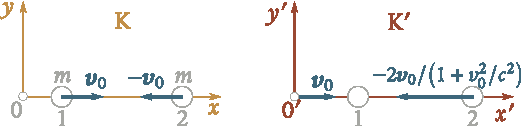
\includegraphics[scale=0.95]{figures/ch_08/fig_8_4.pdf}
		\caption[]{}
		\label{fig:8_4}
	\end{center}
\end{figure}

Giả thử trong hệ $K$ các quả cầu chuyển động ngược nhau dọc theo trục $x$ với các vận tốc có độ lớn như nhau, các hình chiếu lên trục $x$ bằng: $v_{x1}=v_0$ và $v_{x2}=v_0$ ($v_0$ là vận tốc tương đối của các hệ $K$ và $K'$). Trong những điều kiện này, sau va chạm, các quả cầu sẽ đứng yên: $v_{x1}=v_{x2}=0$. Vậy xung lượng toàn phần của hệ cả trước và sau va chạm đều bằng không, nghĩa là trong hệ $K$ xung lượng được bảo toàn

Bây giờ ta xét cũng quá trình đó trong hệ $K'$. Sử dụng công thức thứ nhất trong các công thức~\eqref{eq:8_28} ta tìm được các giá trị $v_{x1}'=0$ và $v_{x2}'=-2v_0/(1+v_0^2/c^2)$ đối với các vận tốc của các quả cầu trước va chạm, và giá trị trùng nhau $v_{x1}'=v_{x2}'=-v_0$ đối với các vận tốc của các quả cầu sau va chạm. Do đó xung lượng tổng cộng trước va chạm là bằng $-2mv_0/(1+v_0^2/c^2)$, còn sau va chạm là bằng $-2mv_0$. Nếu $v_0\ll c$ thì xung lượng của hệ trước va chạm và sau va chạm thực tế là như nhau. Tuy nhiên trong chuyển động của các quả cầu với vận tốc lớn $v_0$ sự khác nhau của các xung lượng đầu và cuối là quá rõ rệt. Vậy, nếu sử dụng biểu thức Newton đối với xung lượng ta đã đi tới kết luận, dường như là trong hệ $K'$ xung lượng không được bảo toàn. Một trong các định luật cơ bản của cơ học --- định luật bào toàn xung lượng --- theo cách diễn đạt của Newton, là không bất biến đối với các biến đổi Lorentz.

It can be shown that the law of momentum conservation will be invariant with respect to the Lorentz transformations at any velocities if we substitute the proper time of a particle $\tau$ for the time $t$ in the classical expression
\begin{equation}\label{eq:8_30}
	\vec{p} = m\vec{v} = m\diff{\vec{r}}{t}.
\end{equation}

\noindent
Consequently, the relativistic expression for the momentum has the form
\begin{equation}\label{eq:8_31}
	\vec{p} = m\diff{\vec{r}}{\tau}.
\end{equation}

\noindent
When $v\ll c$, the length of the proper time of a particle $\deriv{\tau}$ does not virtually differ from the length $\deriv{t}$ measured according to the clock of the frame in which the motion of the particle is being considered [see \eqn{8_21}]. Hence, \eqn{8_31} transforms into the classical expression~\eqref{eq:8_30}.

Remember that $\deriv{\vec{r}}$ in \eqn{8_31} is the displacement of the particle in the reference frame in which the momentum $\vec{p}$ is determined, whereas the length of time $\deriv{\tau}$ is determined on a clock travelling together with the particle.

We get an expression for the momentum through the time $t$ of the frame of reference relative to which the motion of bodies is being observed. By \eqn{8_21}, we have $\deriv{\tau}=\deriv{t}\left(1-v^2/c^2\right)^{1/2}$, where $v$ is the velocity of the body. This substitution in \eqn{8_31} yields
\begin{equation*}
	\vec{p} = \frac{m}{\left(1-v^2/c^2\right)^{1/2}}\diff{\vec{r}}{t}
\end{equation*}

\noindent
or, since $\diffin{\vec{r}}{t}=\vec{v}$:
\begin{equation}\label{eq:8_32}
	\vec{p} = \frac{m\vec{v}}{\left(1-v^2/c^2\right)^{1/2}}.
\end{equation}

Khối lượng $m$ tham gia vào công thức \eqn{8_32} là bất biến và do đó là đại lượng không phụ thuộc vào vận tốc của vật.

Từ \eqn{8_32} suy ra rằng sự phụ thuộc của xung lượng vào vận tốc là phức tạp hơn điều được giả định trong cơ học Newton. Khi $v\ll c$ biểu thức \eqn{8_32} chuyển thành biểu thức Newton $\vec{p}=m\vec{v}$.

Ta chú ý rằng biểu thức \eqn{8_32} cho cách giải thích sau đây mặc dù ít được sử dụng. Xung lượng, cũng như trong cơ học Newton, bằng tích khối lượng của vật với vận tốc của nó:
\begin{equation}\label{eq:8_33}
	\vec{p} = m_{\text{r}}\vec{v}.
\end{equation}

\noindent
Tuy vậy khối lượng của vật không phải là một đại lượng bất biến không đổi mà phụ thuộc vào vận tốc theo định luật
\begin{equation}\label{eq:8_34}
	m_{\text{r}} = \frac{m}{\left(1-v^2/c^2\right)^{1/2}}.
\end{equation}

\noindent
Với sự giải thích như vậy, người ta gọi khối lượng bất biến $m$ là \textbf{khối lượng tĩnh} (thường ký hiệu nó bằng $m_0$). Khối lượng không bất biến $m_{\text{r}}$ phụ thuộc vào vận tốc có tên là \textbf{khối lượng tương đối tính} hoặc \textbf{khối lượng động}.

\section{Biểu thức tương đối tính đối với năng lượng}\label{sec:8_7}

Newton's second law states that the time derivative of the momentum of a particle (point particle) equals the resultant force acting on the particle [see \eqn{2_10}]. The equation of the second law is invariant relative to the Lorentz transformations if by the momentum we understand the quantity~\eqref{eq:8_32}. Hence, the relativistic expression of Newton's second law has the form
\begin{equation}\label{eq:8_35}
	\frac{\upd}{\deriv{t}}\left[\frac{m\vec{v}}{\left(1-v^2/c^2\right)^{1/2}}\right] = \vec{F}.
\end{equation}

It should be borne in mind that the equation $m\vec{a}=\vec{F}$ cannot be used in the relativistic case, the acceleration $\vec{a}$ and the force $\vec{F}$, generally speaking, being non-collinear.

We shall note that neither the momentum nor the force are invariant quantities. Equations for the transformation of the momentum components when passing over from one inertial reference frame to another will be obtained in the following section. We give the equations for transformation of the force components without deriving them:
\begin{equation}\label{eq:8_36}
	F_x = \frac{F_x' + (\beta/c)\vec{F}'\vec{\cdot}\vec{v}'}{1 + \beta(v_x'/c)},\quad F_y = \frac{F_y'\left(1-\beta^2\right)^{1/2}}{1 + \beta(v_x'/c)},\quad F_z = \frac{F_z'\left(1-\beta^2\right)^{1/2}}{1 + \beta(v_x'/c)}
\end{equation}

\noindent
(here $\beta=v_0/c$ and $\vec{v}'$ is the velocity of a particle in the frame K'). If in the frame K$'$ the force $\vec{F}'$ acting on a particle is perpendicular to the velocity of the particle $\vec{v}'$, the scalar product $\vec{F}'\vec{\cdot}\vec{v}'$ equals zero, and the first of the equations~\eqref{eq:8_36} is simplified as follows
\begin{equation}\label{eq:8_37}
	F_x = \frac{F_x'}{1 + \beta(v_x'/c)}.
\end{equation}

\noindent
To find the relativistic expression for the energy, let us proceed in the same way as we did in Sec.~\ref{sec:3_2}. We shall multiply \eqn{8_35} by the displacement of a particle $\deriv{s}=\vec{v}\,\deriv{t}$. The result is
\begin{equation*}
	\frac{\upd}{\deriv{t}}\left[\frac{m\vec{v}}{\left(1-v^2/c^2\right)^{1/2}}\right]\vec{v}\,\deriv{t} = \vec{F}\,\deriv{\vec{s}}.
\end{equation*}

\noindent
The right-hand side of this equation gives the work $\deriv{A}$ done on the particle during the time $\deriv{t}$. We saw in Sec.~\ref{sec:3_2} that the work of the resultant of all the forces is spent on an increment of the kinetic energy of the particle [see \eqn{3_11}]. Consequently, the left-hand side of the equation should be interpreted as the increment of the kinetic energy $E_{\text{k}}$ of the particle during the time $\deriv{t}$. Thus,
\begin{equation*}
	\deriv{E_{\text{k}}} = \frac{\upd}{\deriv{t}}\left[\frac{m\vec{v}}{\left(1-v^2/c^2\right)^{1/2}}\right]\vec{\cdot}\vec{v}\,\deriv{t} = \vec{v}\vec{\cdot} \upd\left[\frac{m\vec{v}}{\left(1-v^2/c^2\right)^{1/2}}\right].
\end{equation*}

Let us transform the obtained expression, bearing in mind that $\vec{v}\vec{\cdot}\deriv{\vec{v}}=\deriv{(\vec{v}^2/2)}$ [see \eqn{1_54}]:
\begin{align*}
	\deriv{E_{\text{k}}} &= \vec{v}\vec{\cdot} \left[\frac{m\,\deriv{\vec{v}}}{\left(1-v^2/c^2\right)^{1/2}} +  \frac{m\vec{v}(\vec{v}\vec{\cdot}\,\deriv{\vec{v}}/c^2)}{\left(1-v^2/c^2\right)^{3/2}}\right]\\
	& = \frac{m\,\deriv{(v^2/2)}}{\left(1-v^2/c^2\right)^{3/2}} = \frac{mc^2\deriv{v^2/c^2}}{2\left(1-v^2/c^2\right)^{3/2}} = \upd\left[\frac{mc^2}{\left(1-v^2/c^2\right)^{1/2}}\right].
\end{align*}

\noindent
Integration of this expression yields
\begin{equation}\label{eq:8_38}
	E_{\text{k}} = \frac{mc^2}{\left(1-v^2/c^2\right)^{1/2}} + \text{constant}.
\end{equation}

\noindent
According to the meaning of kinetic energy, it must vanish when $v=0$. We thus get a value of $-mc^2$ for the constant. Hence, the relativistic expression for the kinetic energy of a particle has the form
\begin{equation}\label{eq:8_39}
	E_{\text{k}} = \frac{mc^2}{\left(1-v^2/c^2\right)^{1/2}} - mc^2 = mc^2\left[\frac{1}{\left(1-v^2/c^2\right)^{1/2}} - 1\right].
\end{equation}

For small velocities ($v\ll c$), \eqn{8_39} can be transformed as follows:
\begin{equation*}
	E_{\text{k}} = mc^2 \left[\frac{1}{\left(1-v^2/c^2\right)^{1/2}} - 1\right]\approx mc^2\left(1 + \frac{1}{2}\frac{v^2}{c^2} - 1\right) = \frac{1}{2}mv^2.
\end{equation*}

\noindent
We have arrived at the Newtonian expression for the kinetic energy of a particle. This is what should be expected because for velocities much smaller than the speed of light all the equations of relativistic mechanics must transform into the relevant equations of Newtonian mechanics.

Let us consider a free particle (\ie, one that does not experience the action of external forces) travelling with the velocity $v$. We have learned that this particle has a kinetic energy determined by \eqn{8_39}. We have grounds, however (see below), to ascribe the additional energy equal to
\begin{equation}\label{eq:8_40}
	E_0 = mc^2
\end{equation}

\noindent
to a free particle in addition to the kinetic energy~\eqref{eq:8_39}. Thus, the total energy of a free particle is determined by the expression $E=E_{\text{k}}+E_0=E_{\text{k}}+mc^2$. With a view to \eqn{8_39}, we find that
\begin{equation}\label{eq:8_41}
	E = \frac{mc^2}{\left(1-v^2/c^2\right)^{1/2}}.
\end{equation}

When $v=0$, \eqn{8_41} transforms into \eqn{8_40}. This is why $E_0=mc^2$ is called the rest energy. This energy is the internal energy of a particle not associated with its motion as a whole. Equations~\eqref{eq:8_40} and~\eqref{eq:8_41} hold not only for an elementary particle, but also for a complicated body consisting of many particles. The energy $E_0$ of such a body includes, apart from the rest energies of its particles, the kinetic energy of these particles (due to their motion relative to the body's centre of mass) and the energy of their interaction with one another. The rest energy, like the total\footnote{We shall note here that the term ``total energy'' has a different meaning in relativistic mechanics than in Newtonian mechanics. In the latter, the total energy is defined as the sum of the kinetic and potential energies of a particle. In relativistic mechanics, by the total energy is meant the sum of the kinetic and rest energies of a particle.} energy~\eqref{eq:8_41}, does not include the potential energy of a body in an external force field.

Eliminating the velocity $v$ from Eqs.~\eqref{eq:8_32} and~\eqref{eq:8_41} [\eqn{8_32} should be taken in the scalar form], we obtain an expression giving the total energy of a particle through its momentum p:
\begin{equation}\label{eq:8_42}
	E = c\left(p^2 + m^2c^2\right)^{1/2}.
\end{equation}

\noindent
When $p\ll mc$, this equation can be written in the form
\begin{equation}\label{eq:8_43}
	E = mc^2\left[1 + \left(\frac{p}{mc}\right)^2\right]\approx mc^2\left[1 + \left(\frac{1}{2}\frac{p}{mc}\right)^2\right] = mc^2 + \frac{p^2}{2m}.
\end{equation}

\noindent
The expression obtained differs from Newton's equation for the kinetic energy $E_{\text{k}}=p^2/(2m)$ in the addend $mc^2$.

It must be noted that the following equation results from a comparison of Eqs.~\eqref{eq:8_32} and~\eqref{eq:8_41}:
\begin{equation}\label{eq:8_44}
	\vec{p} = \frac{E}{c^2}\vec{v}.
\end{equation}

We shall explain why the energy~\eqref{eq:8_41}, and not only the kinetic energy~\eqref{eq:8_39}, should be ascribed to a free particle. Energy according to its meaning must be a conserved quantity. The relevant treatment shows that when particles collide, the sum (for the particles) of expressions of the form of \eqn{8_41} is conserved, whereas the sum of Eqs.~\eqref{eq:8_39} is not conserved. It is impossible to comply with the requirement of energy conservation in all inertial reference frames if we do not include the rest energy~\eqref{eq:8_40} in the total energy.

In addition, we succeed in forming an invariant, \ie, a quantity that does not change in the Lorentz transformations, from \eqn{8_41} for the energy and~\eqref{eq:8_42} for the momentum. Indeed, it can be seen from \eqn{8_42} that
\begin{equation}\label{eq:8_45}
	\frac{E^2}{c^2} - p^2 = m^2c^2 = \text{inv}
\end{equation}

\noindent
(we remind our reader that the mass $m$ and speed $c$ are invariant quantities). Experiments with fast particles confirm the invariance of the quantity in \eqn{8_45}. If by $E$ in \eqn{8_45} we understand the kinetic energy~\eqref{eq:8_39}, then \eqn{8_45} will not be invariant.

Let us obtain another expression for the relativistic energy. From \eqn{8_21}, we find that
\begin{equation}\label{eq:8_46}
	\frac{1}{\left(1 - v^2/c^2\right)^{1/2}} = \diff{t}{\tau}
\end{equation}

\noindent
where $\deriv{t}$ is the time that elapses between two events occurring with a particle and measured on a clock of the reference frame relative to which the particle is travelling with the velocity $v$, while $\deriv{\tau}$ is the same time measured on a clock travelling together with the particle (proper time). Using \eqn{8_46} in \eqn{8_41} we get the expression
\begin{equation}\label{eq:8_47}
	E = mc^2\,\diff{t}{\tau}.
\end{equation}

\noindent
We shall use this equation in the following section.

\section{Transformations of Momentum and Energy}\label{sec:8_8}

The total energy $E$ and momentum $p$ are not invariants. Indeed, both quantities depend on $v$, while the latter has different values in different reference frames. Let us see how the energy and momentum transform when we pass over from one reference frame to another.

Consider an elementary displacement of a particle. Assume that in the reference frame K this displacement occurs during the time $\deriv{t}$, and its components are $\deriv{x}, \deriv{y}, \deriv{z}$. In the frame K$'$, the same displacement occurs during the time $\deriv{t'}$, and its components are $\deriv{x'}, \deriv{y'}, \deriv{z'}$. According to Eqs.~\eqref{eq:8_18}, the following relations hold between the lengths of time and the components of the displacement:
\begin{equation*}
	\deriv{x} = \frac{\deriv{x'}+\beta c\,\deriv{t'}}{\left(1 - \beta^2\right)^{1/2}},\quad \deriv{y}=\deriv{y'},\quad \deriv{z}=\deriv{z'},\quad c\,\deriv{t} = \frac{c\,\deriv{t'}+\beta\,\deriv{x'}}{\left(1 - \beta^2\right)^{1/2}}.
\end{equation*}

Let us multiply these equations by the mass of the particle $m$ and divide them by the proper time of the particle $\deriv{\tau}$ corresponding to the lengths of time $\deriv{t}$ and $\deriv{t'}$ (it should be remembered that the mass and the proper time are invariant quantities, \ie, have the same value in both frames). As a result, we get
\begin{equation}\label{eq:8_48}
	\begin{split}
	&m\,\diff{x}{\tau} = \frac{m(\diffin{x'}{\tau})+\beta mc(\diffin{t'}{\tau})}{\left(1 - \beta^2\right)^{1/2}},\quad m\,\diff{y}{\tau} = m\,\diff{y'}{\tau},\\
	&m\,\diff{z}{\tau} = m\,\diff{z'}{\tau},\quad mc\,\diff{t}{\tau} = \frac{mc(\diffin{t'}{\tau})+\beta m(\diffin{x'}{\tau})}{\left(1 - \beta^2\right)^{1/2}}.
	\end{split}
\end{equation}

By \eqn{8_31}, we have $m\,(\diffin{x}{\tau})=p_x, m\,(\diffin{x'}{\tau})=p_x', m\,(\diffin{y}{\tau})=p_y$, etc. According to \eqn{8_47}, we have $mc\,(\diffin{t}{\tau})=E/c$, and $mc\,(\diffin{t'}{\tau})=E'/c$. Hence, Eqs.~\eqref{eq:8_48} can be written in the form
\begin{equation}\label{eq:8_49}
	p_x = \frac{p_x'+\beta(E'/c)}{\left(1 - \beta^2\right)^{1/2}},\quad p_y = p_y',\quad p_z = p_z',\quad \frac{E}{c} = \frac{(E'/c)+\beta p_x'}{\left(1 - \beta^2\right)^{1/2}}.
\end{equation}

We have obtained equations by means of which the momentum and energy of a particle are transformed when we pass over from one inertial reference frame to another. These equations coincide with Eqs.~\eqref{eq:8_18} used to transform the coordinates and time. To facilitate a comparison, let us write Eqs.~\eqref{eq:8_18} and~\eqref{eq:8_49} side by side:
\begin{equation}\label{eq:8_50}
	\begin{split}
		&x = \frac{x'+\beta(ct')}{\left(1 - \beta^2\right)^{1/2}},\quad y=y',\quad z=z',\quad (ct) = \frac{(ct')+\beta x'}{\left(1 - \beta^2\right)^{1/2}}\\
		&p_x = \frac{p_x'+\beta(E'/c)}{\left(1 - \beta^2\right)^{1/2}},\quad p_y = p_y',\quad p_z = p_z',\quad \frac{E}{c} = \frac{(E'/c)+\beta p_x'}{\left(1 - \beta^2\right)^{1/2}}.
	\end{split}
\end{equation}

\noindent
It follows from the comparison that the components of the momentum behave in transformations like coordinates, and the energy like time.

The analogy disclosed by Eqs.~\eqref{eq:8_50} allows us to present the mathematics of relativistic mechanics in the form of relations between vectors in an imaginary four-dimensional space (four-vectors). We have already noted in Sec.~\ref{sec:8_1} that we have to ascribe unusual properties to this space which differ from the properties of the Euclidean space we are accustomed to. In three-dimensional Euclidean space, the quantity
\begin{equation*}
	\Delta l^2 = \Delta x^2 + \Delta y^2 + \Delta z^2
\end{equation*}

\noindent
is an invariant, \ie, does not change upon rotations of the coordinate axes. Unlike this, the quantity
\begin{equation}\label{eq:8_51}
	c^2\Delta t^2 + \Delta x^2 + \Delta y^2 + \Delta z^2
\end{equation}

\noindent
is not invariant---it is not conserved upon transition from one inertial reference frame to another (such a transition can be imagined as rotation of the axes in four-dimensional space). Hence, the quantity~\eqref{eq:8_51} does not have the properties of the square of the distance between two world points. We have seen in Sec.~\ref{sec:8_4} that \eqn{8_22}, \ie,
\begin{equation*}
	\Delta s^2 = c^2\Delta t^2 - \Delta x^2 - \Delta y^2 - \Delta z^2
\end{equation*}

\noindent
is invariant, and it should be considered as the square of the distance between two points in the four-dimensional space we are interested in\footnote{Naturally, we can also consider Euclidean four-dimensional space. The latter is not suitable for the needs of relativistic mechanics, however.}.

Having given four-dimensional space such properties, we can consider the quantities $ct, x, y, z$ as the components of a four-vector drawn from the origin of coordinates to the given world point. Accordingly, $c\Delta t, \Delta x, \Delta y, \Delta z$ can be considered as components of a four-vector---the displacement from one world point to another. In three-dimensional Euclidean space, other vectors are dealt with (velocity, acceleration, force, etc.) in addition to the position and displacement vectors, and for any vector $\vec{a}$, the quantity
\begin{equation*}
	\vec{a}^2 = a_x^2 + a_y^2 + a_z^2
\end{equation*}

\noindent
is an invariant. The components of any such vector transform upon rotation of the coordinate axes according to the same equations as the coordinates do.

By analogy with three-dimensional vectors in Euclidean space, we can determine four-dimensional vectors. A four-dimensional vector or four-vector is defined as a combination of the four quantities $a_t, a_x, a_y, a_z$ that transform according to the same equations as $ct, x, y, z$ [see the first line of Eqs.~\eqref{eq:8_50}]. The ``square'' of such a vector should be determined as
\begin{equation}\label{eq:8_52}
	a_t^2 - a_x^2 - a_y^2 - a_z^2.
\end{equation}

\noindent
Since the components transform in the same way as the coordinates, expression~\eqref{eq:8_52} is invariant with respect to the Lorentz transformations.

Inspection of Eqs.~\eqref{eq:8_50} shows that the combination of the quantities
\begin{equation}\label{eq:8_53}
	E/c,\, p_x,\, p_y,\, p_z
\end{equation}

\noindent
forms a four-vector. It is called the \textbf{energy-momentum vector}. An expression such as~\eqref{eq:8_52} formed from the components~\eqref{eq:8_53}, as we have established [see \eqn{8_45}], is an invariant:
\begin{equation*}
	\left(\frac{E}{c}\right)^2 - p_x^2 - p_y^2 - p_z^2 = m^2c^2.
\end{equation*}

\section{Relation Between Mass and Energy}\label{sec:8_9}

Using the relativistic mass [see \eqn{8_34}], we can write \eqn{8_41} in the form
\begin{equation}\label{eq:8_54}
	E = m_{\text{r}}c^2.
\end{equation}

\noindent
It can be seen from this equation that the energy of a body and its relativistic mass are always proportional to each other. Any change in the energy of a body $\Delta E$ (except for a change in the potential energy in an external force field) is attended by a change in the relativistic mass of the body $\Delta m_{\text{r}} = \Delta E/c^2$, and, conversely, any change in the relativistic mass $\Delta m_{\text{r}}$ is attended by a change in the energy of the body
\begin{equation}\label{eq:8_55}
	\Delta E = c^2 \Delta m_{\text{r}}.
\end{equation}

\noindent
This statement is called the \textbf{law of the relation between the relativistic mass and energy}\footnote{We sometimes speak of the equivalence of mass and energy having in mind their relation and proportionality to each other.}.

The proportionality between the relativistic mass and energy leads to the fact that the statement on the conservation of the total relativistic mass of particles is the statement on the conservation of the total energy using different words. In this connection, it is not customary practice to speak of the law of relativistic mass conservation as of a separate law.

Unlike the relativistic mass, the total rest mass of a system of interacting particles is not conserved. For example, upon an inelastic collision of two particles observed in the frame of their centre of mass, the rest mass of the particle formed is
\begin{equation*}
	m_{\upSigma} = m_1 + m_2 + \frac{E_{\text{k},1}+E_{\text{k},2}}{c^2}
\end{equation*}

\noindent
where $m_1$ and $E_{\text{k},1}$ are the rest mass and kinetic energy of the first initial particle, and $m_2$ and $E_{\text{k},2}$ are the relevant quantities of the second particle. Thus,
\begin{equation*}
	m_{\upSigma} > m_1 + m_2.
\end{equation*}

\noindent
In this case, the kinetic energy of the initial particles transformed into the internal energy of the formed particle. As a result, the rest mass of this particle exceeded the sum of the rest masses of the initial particles.

The operation of nuclear power plants is based on the chain reaction of fission of nuclei of uranium $\ce{_92U^235}$ (or plutonium) when they capture slow neutrons $n$\footnote{The symbol $\ce{_92U^235}$ stands for the uranium isotope with a mass number of 235. The nucleus of an atom of this isotope consists of $92$ protons and $235-92=143$ neutrons. The symbol $n$ stands for a neutron.}. Fission occurs in various ways. One of the reactions is
\begin{equation}\label{eq:8_56}
	\ce{_92U^235 + }n \ce{-> _92U^236 -> _55Cs^140 + _37Rb^94 + 2}n.
\end{equation}

\noindent
After capturing a neutron, a uranium nucleus decays into a caesium nucleus with the mass number $140$ and a rubidium nucleus with the mass number $94$. Two neutrons are also emitted. The total rest mass of uranium-$235$ and a neutron exceeds the total rest mass of the particles in the right-hand side of the reaction formula~\eqref{eq:8_56} by about \SI{4e-28}{\kilo\gram}. The internal energy corresponding to this surplus mass and equal to
\begin{equation*}
	E = c^2\Delta m = \left(\num{3e8}\right)^2 \times \num{4e-28} \approx \SI{4e-11}{\joule}
\end{equation*}

\noindent
transforms into the kinetic energy of the particles formed (fission fragments) and into the energy of electromagnetic radiation appearing upon fission.

\section{Particles with a Zero Rest Mass}\label{sec:8_10}

Assuming in \eqn{8_42} that $m$ equals zero, we get
\begin{equation}\label{eq:8_57}
	E = cp.
\end{equation}

\noindent
This equation agrees with \eqn{8_44} only if $v=c$. Hence it follows that a particle having a zero rest mass always travels with the speed of light. Such particles include a light particle called a \textbf{photon}, and also elementary particles called \textbf{neutrinos}.

The energy of a photon is determined by the equation
\begin{equation}\label{eq:8_58}
	E = \hbar\omega
\end{equation}

\noindent
where $\hbar$ is Plancks' constant $h$ divided by $2\pi$, and $\omega$ is the cyclic frequency [see \eqn{7_58}].

According to Eqs.~\eqref{eq:8_57} and~\eqref{eq:8_58}, a photon has the momentum
\begin{equation}\label{eq:8_59}
	p = \frac{\hbar\omega}{c}.
\end{equation}

\noindent
Light is a stream of photons. When light is absorbed or reflected from the surface of a body, a momentum is imparted to the latter. This manifests itself in the form of pressure exerted by the light on the body. P.~Lebedev succeeded in discovering and measuring light pressure in 1900. The results of his measurements completely agreed with \eqn{8_59}.

According to Einstein's general theory of relativity, any object having the energy $E$ also has the gravitational mass
\begin{equation*}
	m_{\text{g}} = \frac{E}{c^2}
\end{equation*}

\noindent
\ie, it should be attracted to other objects. Accordingly, a photon should behave in a gravitational field like a particle of the gravitational mass
\begin{equation}\label{eq:8_60}
	m_{\text{g}} = \frac{\hbar\omega}{c^2}.
\end{equation}

\noindent
Particularly, when moving vertically upward near the Earth's surface, a photon must spend part of its energy on doing work against the forces of gravity equal to
\begin{equation*}
	A = m_{\text{g}} gl = \frac{\hbar\omega gl}{c^2}
\end{equation*}

\noindent
where $l$ is the distance travelled. Accordingly, the initial energy of a photon equal to $\hbar\omega$ must diminish by
\begin{equation*}
	\Delta E = \Delta(\hbar\omega) = \frac{\hbar\omega gl}{c^2}.
\end{equation*}

\noindent
Hence,
\begin{equation*}
	\Delta\omega = \frac{\omega gl}{c^2}.
\end{equation*}

\noindent
We thus get the following expression for the relative reduction in the frequency of a photon:
\begin{equation}\label{eq:8_61}
	\frac{\Delta\omega}{\omega} = \frac{gl}{c^2}.
\end{equation}

The change in the frequency of a photon when propagating vertically was measured in 1959 by the U.S. scientists R. Pound and G. Rebka, Jr. Their result coincided with that calculated by \eqn{8_61} with an accuracy of 15\%. We must note that in the conditions of their experiment the relative change in the frequency had a negligibly small value equal to \num{2e-15}.

The effect of the change in the frequency of light when moving away from a large gravitating mass is called the \textbf{gravitational red shift}. The meaning of this term will be disclosed in the third volume of the present course.
